\documentclass[utf8x,xcolor=pdftex,dvipsnames,table]{beamer}
\usetheme{Malmoe}  % Now it's a beamer presentation with the lisa theme!
\setbeamertemplate{footline}[page number]
\usecolortheme{beaver}
\usepackage[T1]{fontenc}
\usepackage{amsmath}
\usepackage[utf8x]{inputenc}
\usepackage{multicol}
%\logo{
\includegraphics[width=.8in]{UdeM_NoirBleu_logo_Marie_crop}}
\usepackage{listings}

\newcommand{\superscript}[1]{\ensuremath{^{\textrm{#1}}}}

\mode<presentation>

\title{Theano at a Glance:\newline A Framework for Machine Learning}

\author{%
\footnotesize
Frédéric Bastien \newline
\newline
\newline
Montreal Institute for Learning Algorithms \newline
Université de Montréal \newline
Montréal, Canada \newline
\texttt{bastienf@iro.umontreal.ca} \newline \newline
Presentation prepared with Pascal Lamblin and Simon Lefrancois
}

\date{NYCPython meetup 2017}

\setbeamertemplate{navigation symbols}{}
\begin{document}

\begin{frame}[plain]
 \titlepage
 \vspace{-5em}
 
\includegraphics[width=1.1in]{../pics/MILA.png}
 \hfill
 
\includegraphics[width=.8in]{../pics/UdeM_NoirBleu_logo_Marie_crop}
\end{frame}

\section{Introduction}
\subsection{Introduction}
\begin{frame}
  \tableofcontents[currentsection]
\end{frame}

\begin{frame}{High level}  %\setcounter{page}{1}
  Python <- \{NumPy/SciPy/libgpuarray\} <- Theano <- \{...\}
  \begin{itemize}
  \item Python: OO coding language
  \item Numpy: $n$-dimensional array object and scientific computing toolbox
  \item SciPy: sparse matrix objects and more scientific computing functionality
  \item libgpuarray: GPU $n$-dimensional array object in C for CUDA and OpenCL
  \item Theano: compiler/symbolic graph manipulation
    \begin{itemize}
    \item \bf{(Not specific to machine learning)}
    \end{itemize}
  \item \{...\}: Many libraries built on top of Theano

  \end{itemize}
\end{frame}

\begin{frame}{What Theano provides}
  \begin{itemize}
    \item Lazy evaluation for performance
    \item GPU support
    \item Symbolic differentiation
    \item Automatic speed and stability optimization
  \end{itemize}

\end{frame}

\begin{frame}{High level}
  Many [machine learning] library build on top of Theano
  \begin{itemize}
  \item Keras
  \item blocks
  \item lasagne
  \item sklearn-theano
  \item PyMC 3
  \item theano-rnn
  \item Morb
  \item ...
  \end{itemize}
\end{frame}

\begin{frame}{Goal of the stack}
\begin{center}
\begin{bf}Fast to develop\end{bf}\newline \bigskip
\begin{bf}Fast to run\end{bf}\newline \bigskip
\hspace{-2.5cm}
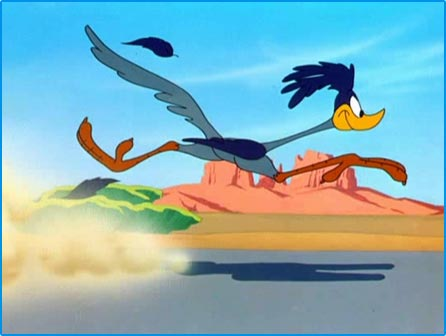
\includegraphics[width=0.35\textwidth]{../pics/road-runner-1.jpg}
\end{center}
\end{frame}

\begin{frame}{Some models build with Theano}
  Some models that have been build with Theano.
  \begin{itemize}
  \item Neural Networks
  \item Convolutional Neural Networks, AlexNet, OverFeat, GoogLeNet
  \item RNN, CTC, LSTM, GRU
  \item NADE, RNADE, MADE
  \item Autoencoders
  \item Generative Adversarial Nets
  \item SVMs
  \item \begin{bf}many variations of above models and more\end{bf}
  \end{itemize}
\end{frame}

%% \begin{frame}{Others}
%%   \begin{itemize}
%%   \item IPython: Advanced python shell
%%   \item IPython notebook: web-based interactive computational environment where you can combine code execution, text, mathematics, plots and rich media into a single document
%%   \item matplotlib: one of the many plotting library
%%  \item PyTables: hdf5 container with extra functionality
%%  \item pandas: other data structure
%%  \item ...
%%   \end{itemize}
%% \end{frame}

\begin{frame}{Project status}
  \begin{itemize}
    \item Mature: Theano has been developed and used since January 2008 (9 yrs old)
    \item Driven hundreds of research papers % Over a thousands of research paper
    \item Good user documentation
    \item Active mailing list with worldwide participants
    \item Core technology for Silicon-Valley start-ups
    \item Many contributors (some from outside our institute)
    \item Used to teach many university classes
    \item Used for research at big compagnies
    \item Theano 0.9 released 20th of March, 2017
  \end{itemize}
  Theano: \url{deeplearning.net/software/theano/}

  Deep Learning Tutorials: \url{deeplearning.net/tutorial/}
\end{frame}

%%TODO: slide MILA
%%Institut des algorithmes d'apprentissage de Montréal
%%Montreal Institute for Learning Algorithms

%%- TODOWho we are, what we do
\subsection{Community}
\begin{frame}{Theano community}
Active community
  \begin{itemize}
  \item Many people reply on our mailing lists
  \item Hundreds of answered questions on StackOverflow
  \item 123 contributors to Theano 0.9
  \item Main developers at MILA
  \end{itemize}
\end{frame}

\begin{frame}{MILA}
Institut des algorithmes d'apprentissage de Montréal\newline
Montreal Institute for Machine Learning\newline
\begin{itemize}
\item Professors 8
\item Staff 11
\item Visiting Scientists 1
\item Post-Doc 9
\item Ph.D. students 46
\item M.Sc. students 23
\item Interns 15
\item Total 113
\end{itemize}
 \vspace{-5em}
 \hspace{19em}
 
\includegraphics[width=1.4in]{../pics/MILA.png}
 \hfill
\url{mila.umontreal.ca} \newline
\begin{tiny}formely known as LISA\end{tiny}
\end{frame}

\begin{frame}{MILA Partners}
    \begin{multicols}{2}
  \begin{itemize}
    
\item Many universities
\item Nuance
\item IBM
\item Google
\item Facebook
\item NVIDIA
\item Huawei
\item amazon.com
\item Druide
\item Microsoft
\item Intel
\item D-Wave
\item ApSTAT
\item Qualcomm
\item Imagia
\item Sulfur Heron
\item Ubisoft
    \end{itemize}

\end{multicols}
\end{frame}


\section{Theano}
\subsection{Description}

%% \begin{frame}{Python}
%%   \begin{itemize}
%%   \item General-purpose high-level OO interpreted language
%%   \item Emphasizes code readability
%%   \item Comprehensive standard library
%%   \item Dynamic type and memory management
%%   \item Easily extensible with C
%%   \item Slow execution
%%   \item Popular in {\em web development}\ and {\em scientific communities}
%%   \end{itemize}
%% \end{frame}

\begin{frame}
  \tableofcontents[currentsection]
\end{frame}

%\subsection{Introduction}
\begin{frame}{Description}

  High-level domain-specific language for numeric computation.

  \begin{itemize}
    \item \begin{bf}Syntax as close to NumPy\end{bf} as possible
    \item \begin{bf}Compiles\end{bf} most common expressions \begin{bf}to C for CPU and/or GPU\end{bf}
    \item \begin{bf}Limited expressivity\end{bf} means more opportunities for optimizations
    \begin{itemize}
      \item \begin{bf}Strongly typed\end{bf} -> compiles to C
      \item \begin{bf}Array oriented\end{bf} -> easy parallelism
      \item Support for \begin{bf}looping and branching\end{bf} in expressions
      \item No subroutines -> \begin{bf}global optimization\end{bf}
    \end{itemize}
    \item \begin{bf}Automatic\end{bf} speed and numerical stability \begin{bf}optimizations\end{bf}
  \end{itemize}
\end{frame}

\begin{frame}{Description (2)}

  \begin{itemize}
    \item \begin{bf}Symbolic differentiation and R op\end{bf} (Hessian Free Optimization)
    \item Can \begin{bf}reuse other technologies\end{bf} for best performance
    \begin{itemize}
      \item CUDA, CuBLAS, CuDNN, BLAS, SciPy, PyCUDA, Cython, Numba, ...
    \end{itemize}
    \item Works on \begin{bf}Linux, OS X and Windows\end{bf}
    \item \begin{bf}Multi-GPU\end{bf} (via platoon)
    \item New GPU back-end:
      \begin{itemize}
      \item \begin{bf}Float16\end{bf} new back-end (need cuda 7.5)
      \item \begin{bf}Multi dtypes\end{bf}
%      \item Multi-GPU support in the same process
      \end{itemize}
    \item Sparse matrices (CPU only)
    \item Extensive unit-testing and self-verification
    \item Extensible (You can create new operations as needed)
  \end{itemize}
\end{frame}



%% \begin{frame}{Why scripting for GPUs?}
%%   \begin{bf}They complement each other\end{bf}

%%   GPUs are everything that high level languages are not

%%   \begin{itemize}
%%     \item Highly parallel
%%     \item Very architecture-sensitive
%%     \item Built for maximum FP/memory throughput
%%     \item So hard to program that meta-programming is easier
%%   \end{itemize}

%%   \begin{bf}Best of both worlds:\end{bf} easily scripted code which invokes high-performance GPU kernels.

%%   \begin{bf}Theano C code generation removes overhead\end{bf} of
%%   function calls between Python and C by launching many C functions at once.

%% \end{frame}

%\subsection{Simple Example}
\begin{frame}[fragile]
  \frametitle{Simple example}

\lstset{language=Python,
        commentstyle=\itshape\color{blue},
        stringstyle=\color{violet},
        }
\begin{lstlisting}
import theano
# declare symbolic variable
a = theano.tensor.vector("a")

# build symbolic expression
b = a + a ** 10

# compile function
f = theano.function([a], b)

# Execute with numerical value
print f([0, 1, 2])
# prints `array([0, 2, 1026])`
\end{lstlisting}
\end{frame}

\begin{frame}{Simple example}
\center
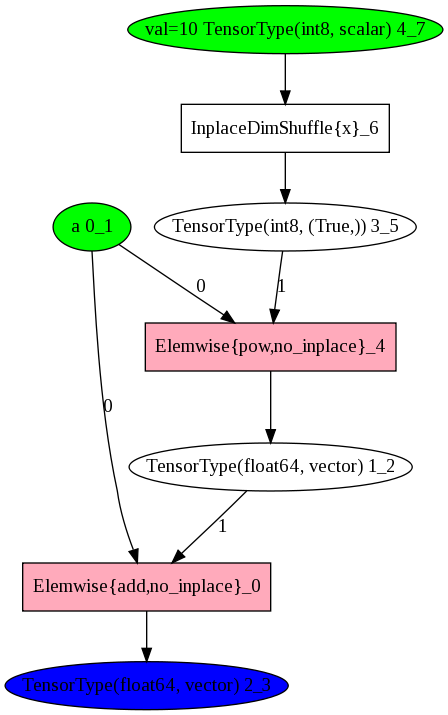
\includegraphics[width=0.35\textwidth]{../pics/f_unoptimized.png}
\hspace{0.1\textwidth}
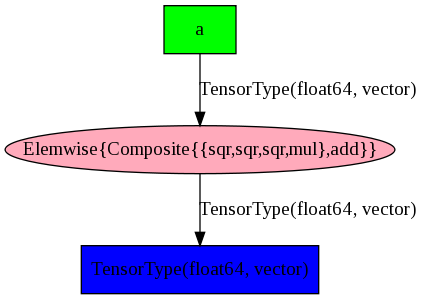
\includegraphics[width=0.35\textwidth]{../pics/f_optimized.png}
\end{frame}


\begin{frame}{Overview of library}
  Theano is many things
  \begin{itemize}
  \item Language
  \item Compiler
  \item Python library
  \end{itemize}
\end{frame}

%\subsection{Operations}
%% \begin{frame}{Overview Language}
%%   Most of NumPy and more!
%%   \begin{itemize}
%%   \item Operations on scalars, vectors, matrices, tensors, and sparse variables
%%   \item Linear algebra
%%   \item Element-wise nonlinearities
%%   \item Convolution
%%   \item Indexing, slicing and advanced indexing.
%%   \item Reduction
%%   \item Dimshuffle (n-dim transpose)
%%   \end{itemize}
%% \end{frame}


\subsection{Compiling/Running}
\begin{frame}{Compiling and running expression}
  \begin{itemize}
  \item theano.function
  \item shared variables and updates
  \item compilation modes
%  \item TODO: optimizations
  \end{itemize}
\end{frame}

\begin{frame}[fragile]
  \frametitle{Shared variable example}

\lstset{language=Python,
        commentstyle=\itshape\color{blue},
        stringstyle=\color{violet},
        }
\begin{lstlisting}
>>> from theano import shared
>>> x = shared(0.)  # Normally, model parameters
>>> updates = [(x, x + 1)]
>>> f = function([], updates=updates)
>>> f()
>>> x.get_value()
1.0
>>> x.set_value(100.)
>>> f()
>>> x.get_value()
101.0
\end{lstlisting}
\end{frame}


\subsection{Modifying expressions}
\begin{frame}{Modifying expressions}
  There are ``macro'' that automatically build bigger graph for you.
  \begin{itemize}
  \item theano.grad
  \item R\_op, L\_op for Hessian Free Optimization
  \item hessian
  \item jacobian
  \item clone the graph with replacement
  \item you can navigate the graph if you need
  \end{itemize}
  Those functions can get called many times, for example to get the 2nd
  derivative.
\end{frame}


\begin{frame}[fragile]
  \frametitle{The grad method}
\lstset{language=Python,
        commentstyle=\itshape\color{gray},
        stringstyle=\color{gray},
        keywordstyle=\color{gray},
        rulecolor=\color{gray},
        identifierstyle=\color{gray},
        basicstyle=\color{gray},
        }
\begin{lstlisting}
>>> x = T.scalar('x')
>>> cost = 2. * x
>>> g = T.grad(cost, x)
\end{lstlisting}
\lstset{language=Python,
        commentstyle=\itshape\color{blue},
        stringstyle=\color{violet},
        keywordstyle=\color{black},
        rulecolor=\color{black},
        identifierstyle=\color{black},
        basicstyle=\color{black},
        }
\begin{lstlisting}
# Print the optimized graph
>>> f = theano.function([x], g)
>>> theano.printing.pydotprint(f)
\end{lstlisting}
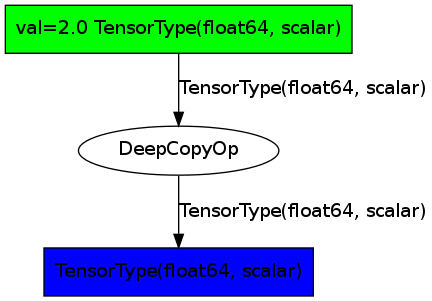
\includegraphics[width=0.4\textwidth]{../pics/theano_grad_opt.png}
\end{frame}

\subsection{GPU}
\begin{frame}{Enabling GPU}
  \begin{itemize}
  \item libgpuarray (new-backend) supports all dtype
  \item Theano's old GPU back-end only supports 32 bit on GPU
  \item CUDA supports float64, but it is slow on gamer GPUs
  \end{itemize}
\end{frame}


\begin{frame}{CuDNN}
  \begin{itemize}
  \item V5 and V5.1 are supported.
  \item V6 compile.
  \item It is enabled automatically if available.
  \item Theano flag to get an error if can't be used: ``dnn.enabled=True''
  \item Theano flag to disable it: ``dnn.enabled=False''
  \end{itemize}
\end{frame}

\subsection{Debugging}
\begin{frame}{Debugging}
  \begin{itemize}
  \item DebugMode: a mode that tests many things done by Theano (very slow)
  \item NanGuardMode: a mode that help find the cause of nan in the graph.
  \item Error message
  \item theano.printing.debugprint: print a textual representation of computation
  \end{itemize}
\end{frame}

\begin{frame}[fragile]
  \frametitle{Error message: code}
\lstset{language=Python,
        commentstyle=\itshape\color{blue},
        stringstyle=\color{violet},
        }
\begin{lstlisting}
import numpy as np
import theano
import theano.tensor as T
x = T.vector()
y = T.vector()
z = x + x
z = z + y
f = theano.function([x, y], z)
f(np.ones((2,)), np.ones((3,)))
\end{lstlisting}
\end{frame}

\begin{frame}[fragile]
  \frametitle{Error message: 1st part}

\lstset{language=Python,
        commentstyle=\itshape\color{blue},
        stringstyle=\color{violet},
        basicstyle=\scriptsize
        }
\begin{lstlisting}
Traceback (most recent call last):
[...]
ValueError: Input dimension mis-match.
    (input[0].shape[0] = 3, input[1].shape[0] = 2)
Apply node that caused the error:
   Elemwise{add,no_inplace}(<TensorType(float64, vector)>,
                            <TensorType(float64, vector)>,
                            <TensorType(float64, vector)>)
Inputs types: [TensorType(float64, vector),
               TensorType(float64, vector),
               TensorType(float64, vector)]
Inputs shapes: [(3,), (2,), (2,)]
Inputs strides: [(8,), (8,), (8,)]
Inputs values: [array([ 1.,  1.,  1.]),
                array([ 1.,  1.]),
                array([ 1.,  1.])]
Outputs clients: [['output']]
\end{lstlisting}
\end{frame}

\begin{frame}[fragile]
  \frametitle{Backtrace}

\lstset{language=Python,
        commentstyle=\itshape\color{blue},
        stringstyle=\color{violet},
        }
\begin{lstlisting}
Backtrace when the node is created:
  File "test.py", line 7, in <module>
    z = z + y

\end{lstlisting}
\end{frame}


\begin{frame}[fragile]
  \frametitle{Error message: 2nd part}
\begin{color}{gray}
HINT: Re-running with most Theano optimization
disabled could give you a back-traces when this
node was created. This can be done with by setting
the Theano flags ``optimizer=fast\_compile''. If that does not
work, Theano optimizations can be disabled with
``optimizer=None''.\newline
\end{color}
HINT: Use the Theano flag ``exception\_verbosity=high''
for a debugprint of this apply node.
\end{frame}


\begin{frame}[fragile]
  \frametitle{debugprint}

\lstset{language=Python,
        commentstyle=\itshape\color{blue},
        stringstyle=\color{violet},
        }
\begin{lstlisting}
>>> from theano.printing import debugprint
>>> debugprint(a)
Elemwise{mul,no_inplace} [id A] ''
 |TensorConstant{2.0} [id B]
 |Elemwise{add,no_inplace} [id C] 'z'
   |<TensorType(float64, scalar)> [id D]
   |<TensorType(float64, scalar)> [id E]
\end{lstlisting}
\end{frame}

\section{Models}
\subsection{Logistic Regression}
\begin{frame}
  \tableofcontents[currentsection]
\end{frame}


\begin{frame}[fragile]
  \frametitle{Inputs}
\lstset{language=Python,
        commentstyle=\itshape\color{blue},
        stringstyle=\color{violet},
        }
\begin{lstlisting}
# Load from disk and put in shared variable.
datasets = load_data(dataset)
train_set_x, train_set_y = datasets[0]
valid_set_x, valid_set_y = datasets[1]

# allocate symbolic variables for the data
index = T.lscalar()  # index to a [mini]batch

# generate symbolic variables for input minibatch
x = T.matrix('x')  # data, 1 row per image
y = T.ivector('y')  # labels
\end{lstlisting}
\end{frame}


\begin{frame}[fragile]
  \frametitle{Model}
\lstset{language=Python,
        commentstyle=\itshape\color{blue},
        stringstyle=\color{violet},
        }
\begin{lstlisting}
n_in = 28 * 28
n_out = 10

# weights
W = theano.shared(
        numpy.zeros((n_in, n_out),
                    dtype=theano.config.floatX))

# bias
b = theano.shared(
        numpy.zeros((n_out,),
                    dtype=theano.config.floatX))
\end{lstlisting}
\end{frame}


\begin{frame}[fragile]
  \frametitle{Computation}
\lstset{language=Python,
        commentstyle=\itshape\color{blue},
        stringstyle=\color{violet},
        }
\begin{lstlisting}
# the forward pass
p_y_given_x = T.nnet.softmax(T.dot(input, W) + b)

# cost we minimize: the negative log likelihood
l = T.log(p_y_given_x)
cost = -T.mean(l[T.arange(y.shape[0]), y])

# the error
y_pred = T.argmax(p_y_given_x, axis=1)
err = T.mean(T.neq(y_pred, y))
\end{lstlisting}
\end{frame}


\begin{frame}[fragile]
  \frametitle{Gradient and updates}
\lstset{language=Python,
        commentstyle=\itshape\color{blue},
        stringstyle=\color{violet},
        }
\begin{lstlisting}
# compute the gradient of cost
g_W, g_b = T.grad(cost=cost, wrt=(W, b))

# model parameters updates rules
updates = [(W, W - learning_rate * g_W),
           (b, b - learning_rate * g_b)]
\end{lstlisting}
\end{frame}


\begin{frame}[fragile]
  \frametitle{Training function}
\lstset{language=Python,
        commentstyle=\itshape\color{blue},
        stringstyle=\color{violet},
        }
\begin{lstlisting}
# compile a Theano function that train the model
train_model = theano.function(
    inputs=[index], outputs=(cost, err),
    updates=updates,
    givens={
        x: train_set_x[index * batch_size:
                       (index + 1) * batch_size],
        y: train_set_y[index * batch_size:
                       (index + 1) * batch_size]
    }
)
\end{lstlisting}
\end{frame}


\subsection{Convolution}
\begin{frame}[fragile]
  \frametitle{Convolution computation}
\lstset{language=Python,
        commentstyle=\itshape\color{blue},
        stringstyle=\color{violet},
        }
\begin{lstlisting}
# convolve input feature maps with filters
conv_out = conv.conv2d(input=x, filters=W)

# pool each feature map individually,
# using maxpooling
pooled_out = pool.pool_2d(
    input=conv_out,
    ds=(2, 2),  # poolsize
    ignore_border=True)

output = T.tanh(pooled_out +
                b.dimshuffle('x', 0, 'x', 'x'))
\end{lstlisting}
\end{frame}


\subsection{Scan}
\begin{frame}
  \frametitle{Scan}
\begin{itemize}
\item Allows looping (for, map, while)
\item Allows recurrence (reduce)
\item Allows recurrence with dependency on a fixed number of previous time steps
\item Optimize some cases like moving computation outside of scan
\item The Scan grad is done via Backpropagation Through Time (BPTT)
\end{itemize}
\end{frame}

\iffalse
\begin{frame}{When not to use scan}
\begin{itemize}
\item If you only need it for ``vectorization'' or
  ``broadcasting''. tensor and numpy.ndarray support them
  natively. This will be much better for that use case.

\item If you do a fixed number of iteration that is very small (2,3). You
  are probably better to just unroll the graph to do it.

\end{itemize}
\end{frame}

\fi

\section{News}
\begin{frame}{Theano 0.9}
\begin{tiny}Released 20th of March, 2017\end{tiny}

Some Highlights:
\begin{itemize}
\item Faster compilation and execution
\item conda packages for Mac, Linux and Windows
\item Bool dtype support
\item Many Scan improvements (execution speed up, checkpoints, ...)
\item Multi-GPU for data parallism via Platoon \url{https://github.com/mila-udem/platoon}
\item New GPU back-end
\item ...
\end{itemize}

A total of 141 people contributed to this release.
\end{frame}


%% \begin{frame}{Since last release}

%% Highlights:
%% \begin{itemize}
%% \item Computation and compilation speed up
%% \item Multi-cores convolution and pooling on CPU
%% \item More numerical stability by default for some graphs
%% \end{itemize}
%% \begin{itemize}
%% \item CuDNN: 5.1, batch normalization, (RNN soon)
%% \item Dilated convolution
%% \item Multiple-GPU, synchronous update (via platoon)
%% \item Partial function evaluation
%% \item Add gradient of solve, tensorinv (CPU), tensorsolve (CPU) searchsorted (CPU)
%% \item Add Multinomial Without Replacement
%% \item ...
%% \end{itemize}
%% 90 people already contributed to the development version.

%% \end{frame}

\begin{frame}{Roadmap}
  \normalsize
  \begin{itemize}
  \item Remove the old GPU back-end
  \item Still Faster compile time
    \begin{itemize}
    \item First time compilation (less C code compilations, already cached)
    \item Of big graph (faster graph optimization)
    \end{itemize}
  \item Handling of bigger graph
  \item Speed/Memory trade off
    \begin{itemize}
    \item Recompute cheap operation of the forward during the gradient
    \end{itemize}
  \item Faster computation (CuDNN v6, ...)
  \item More determinism vs speed tradeoff
  \item Encapsulation of sub graph and redefinition of gradient: OpFromGraph
  \item More variants of convolutions
  \end{itemize}
\end{frame}


\section{End}
\begin{frame}{Where to learn more}
\normalsize
\begin{itemize}
\item Deep Learning Tutorials with Theano: \url{deeplearning.net/tutorial}
\item Theano tutorial: \url{deeplearning.net/software/theano/tutorial}
\item Theano website: \url{deeplearning.net/software/theano}
\item Doc of frameworks on top of Theano like Blocks, Keras, Lasagne, ...
\end{itemize}

\end{frame}

\begin{frame}{Questions, acknowledgments}
\Huge
\begin{center}
Questions?\newline
Acknowledgments
\end{center}
\normalsize
\begin{itemize}
\item All people working or having worked at MILA institute (previously LISA lab).
\item All Theano users/contributors.
\item Compute Canada, RQCHP, NSERC, NVIDIA, and Canada Research Chairs for providing funds, access to computing resources, hardware or GPU libraries.
\end{itemize}

\end{frame}


\end{document}
